%% Additional packages

\documentclass[a4paper]{article}
\usepackage{fontspec}
\usepackage{graphicx}
\usepackage{hyperref}
\usepackage[margin=1.5cm]{geometry}
\usepackage{amsmath}

%% Title

\title{\textbf{Symulacja ruchu ludzi w centrum handlowym}}
\author{Paweł Kłeczek \and Kajetan Rzepecki}
\date{2012-11-01}


%% Text starts here:
\begin{document}

    \vspace{\fill}
    \maketitle
    \vspace{\fill}
    \thispagestyle{empty}

\newpage
    \setcounter{page}{1}
    \setcounter{tocdepth}{3}
    \tableofcontents

\newpage
    \section{Wprowadzenie}
    \label{sec-1}

    \begin{center}
        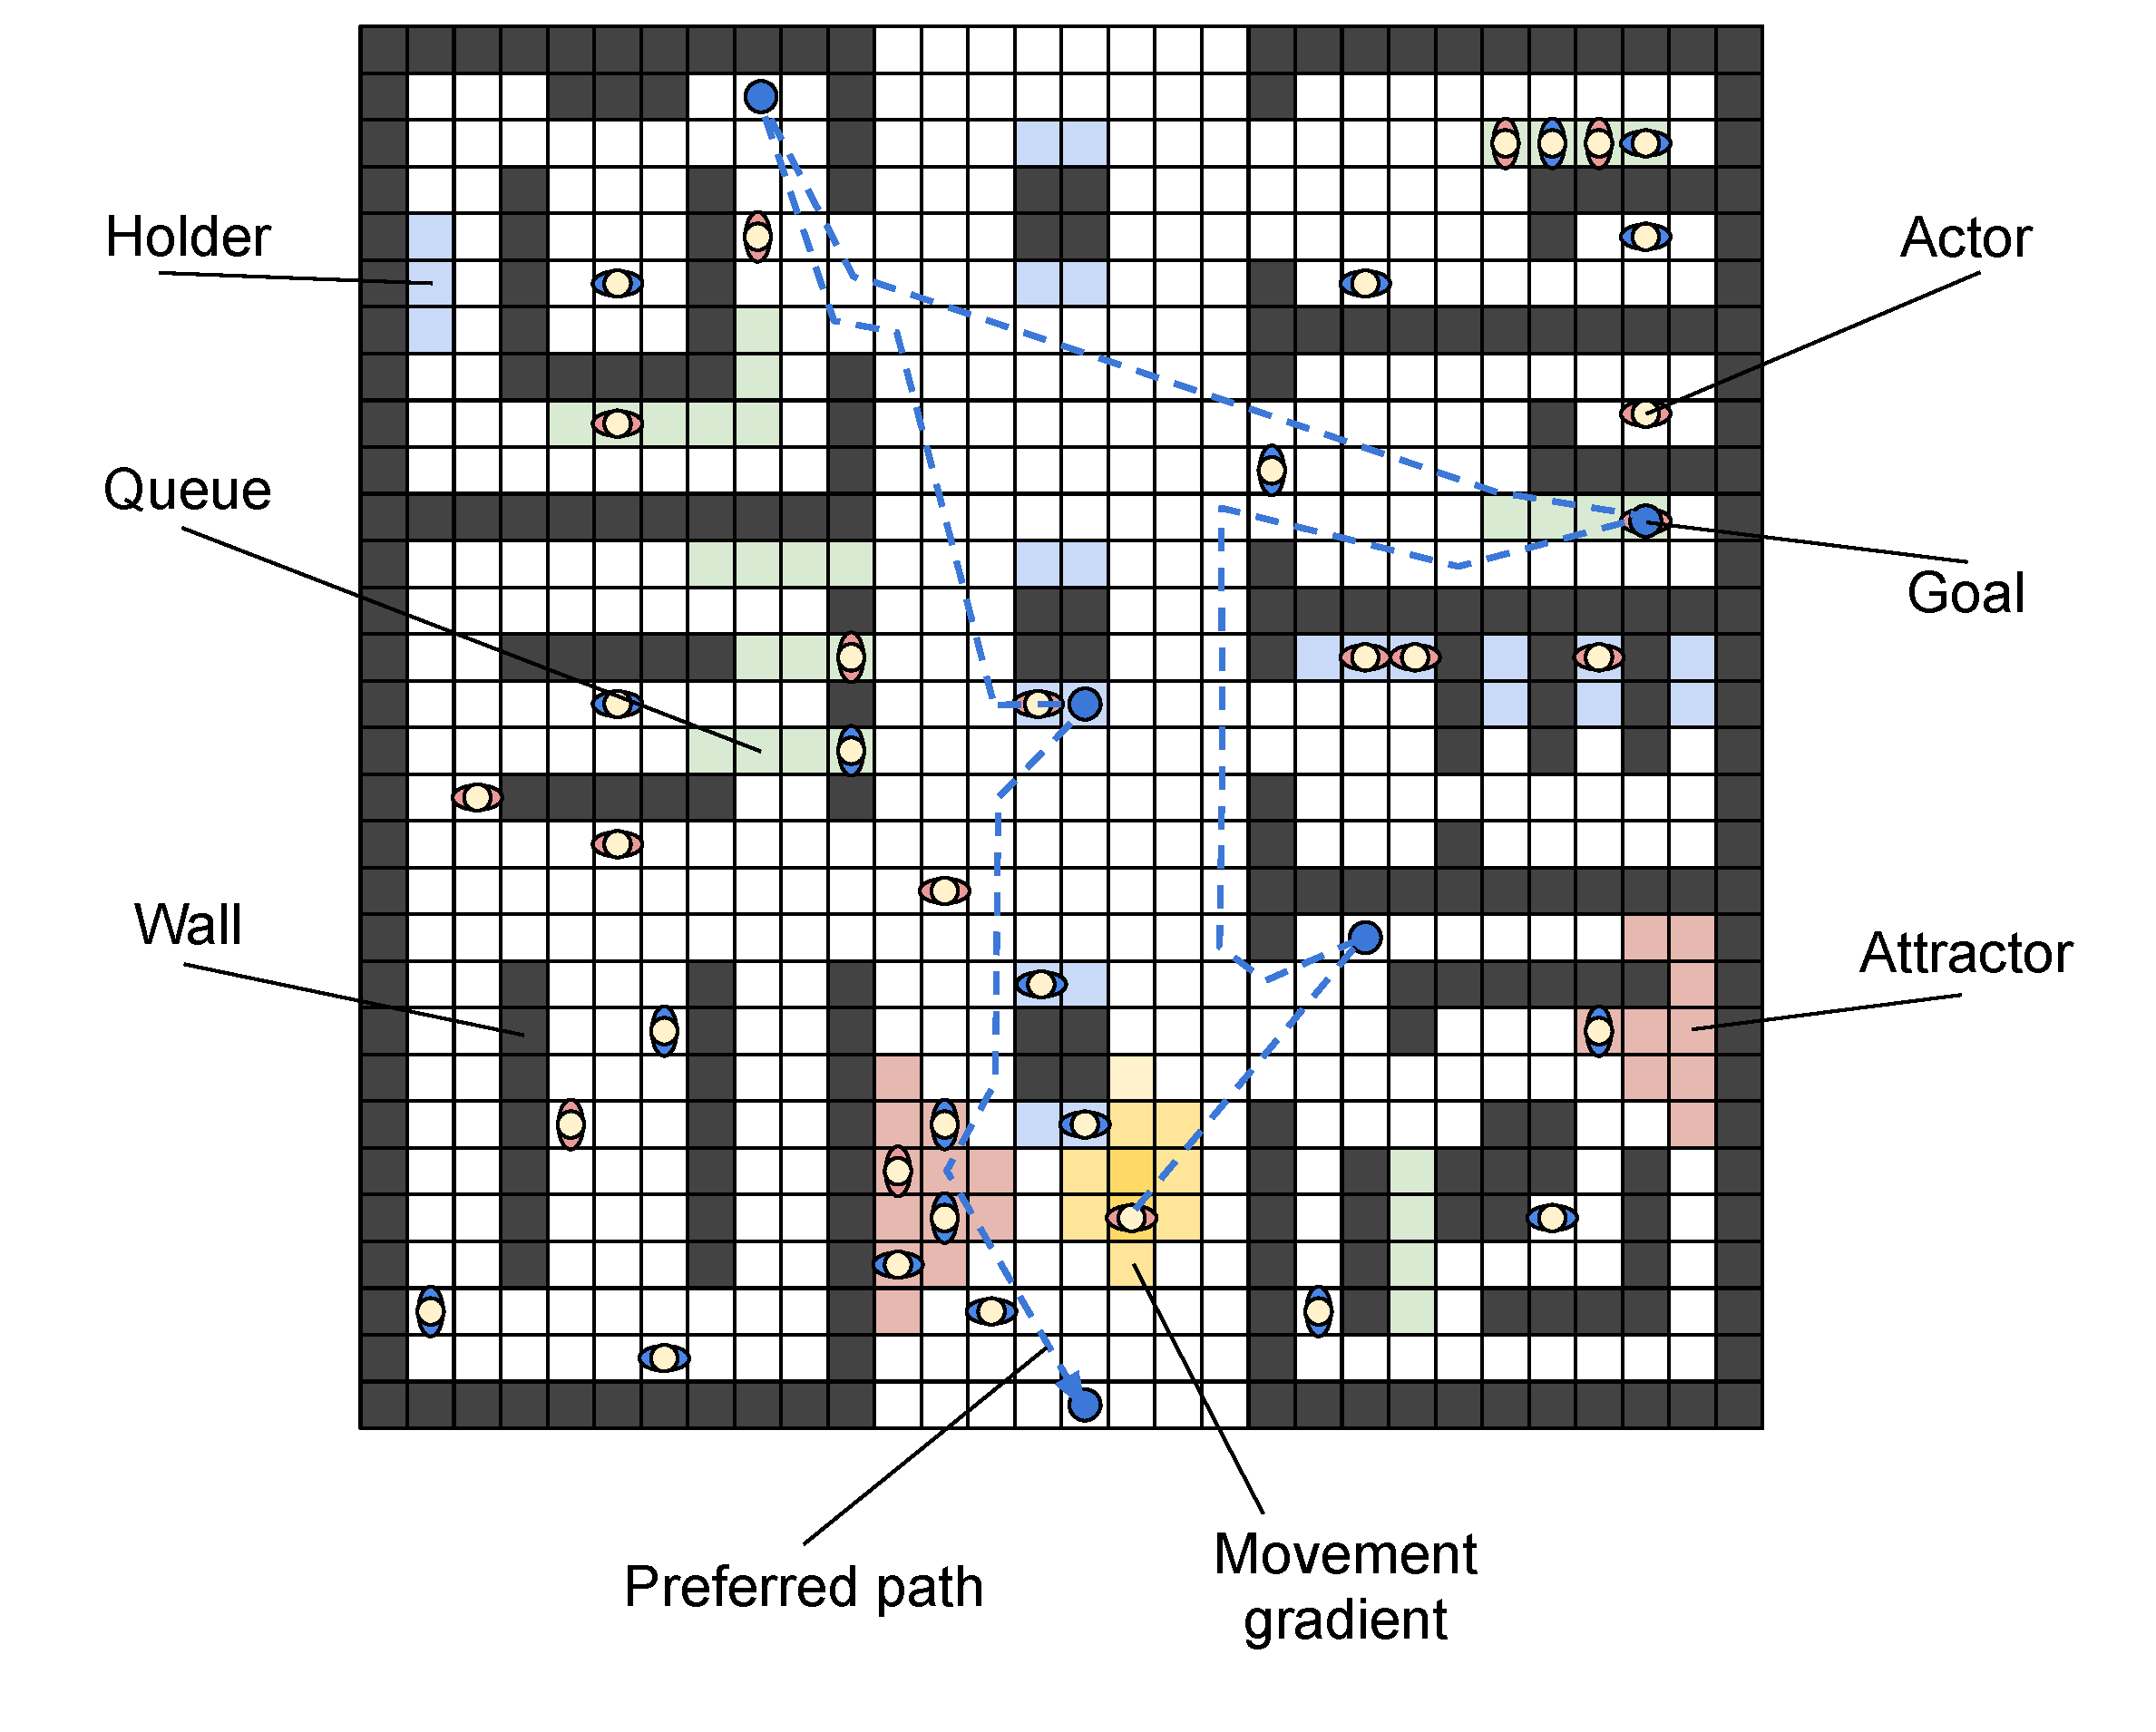
\includegraphics[scale=0.3]{./img/Overview.pdf}
    \end{center}

\noindent
Opis comming soon...

\newpage
    \section{Model ruchu ludzi}
    \label{sec-2}

        \subsection{Poziom taktyczny}
        \label{sec-2-1}

        \begin{center}
            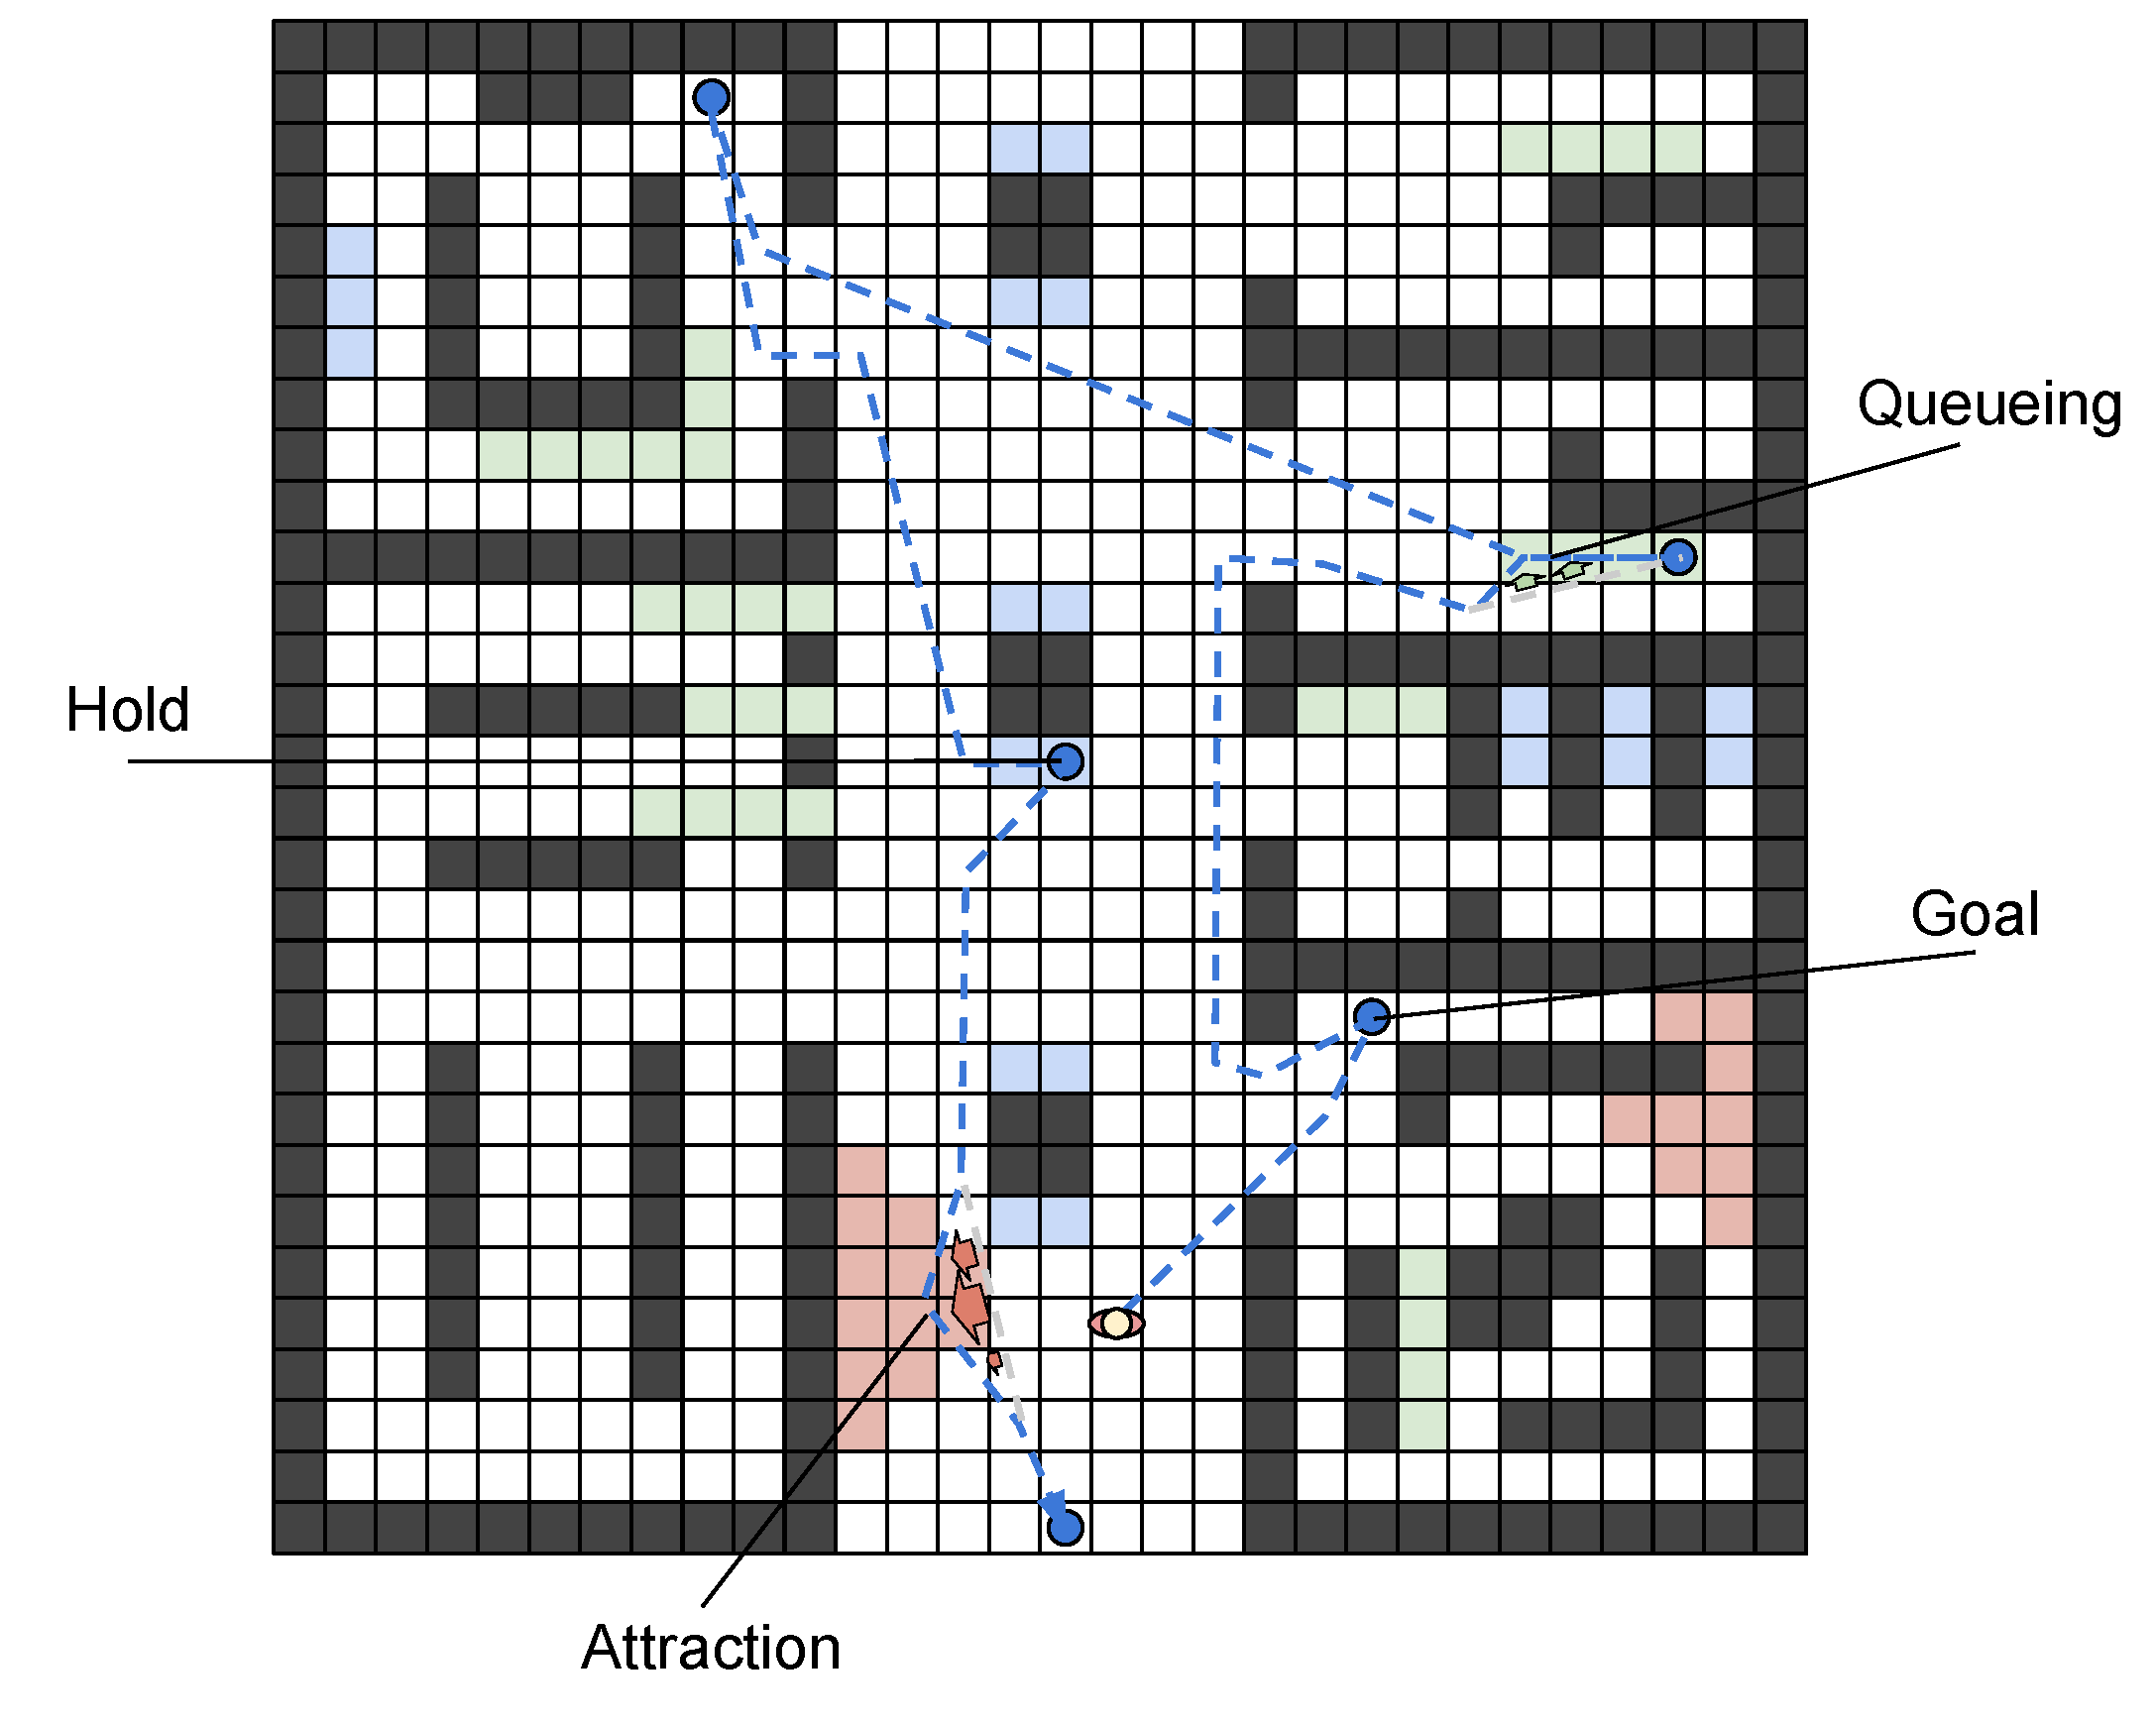
\includegraphics[scale=0.3]{./img/Tactical.pdf}
        \end{center}

\noindent
Opis comming soon...

        \subsection{Poziom operacyjny}
        \label{sec-2-2}

        \begin{center}
            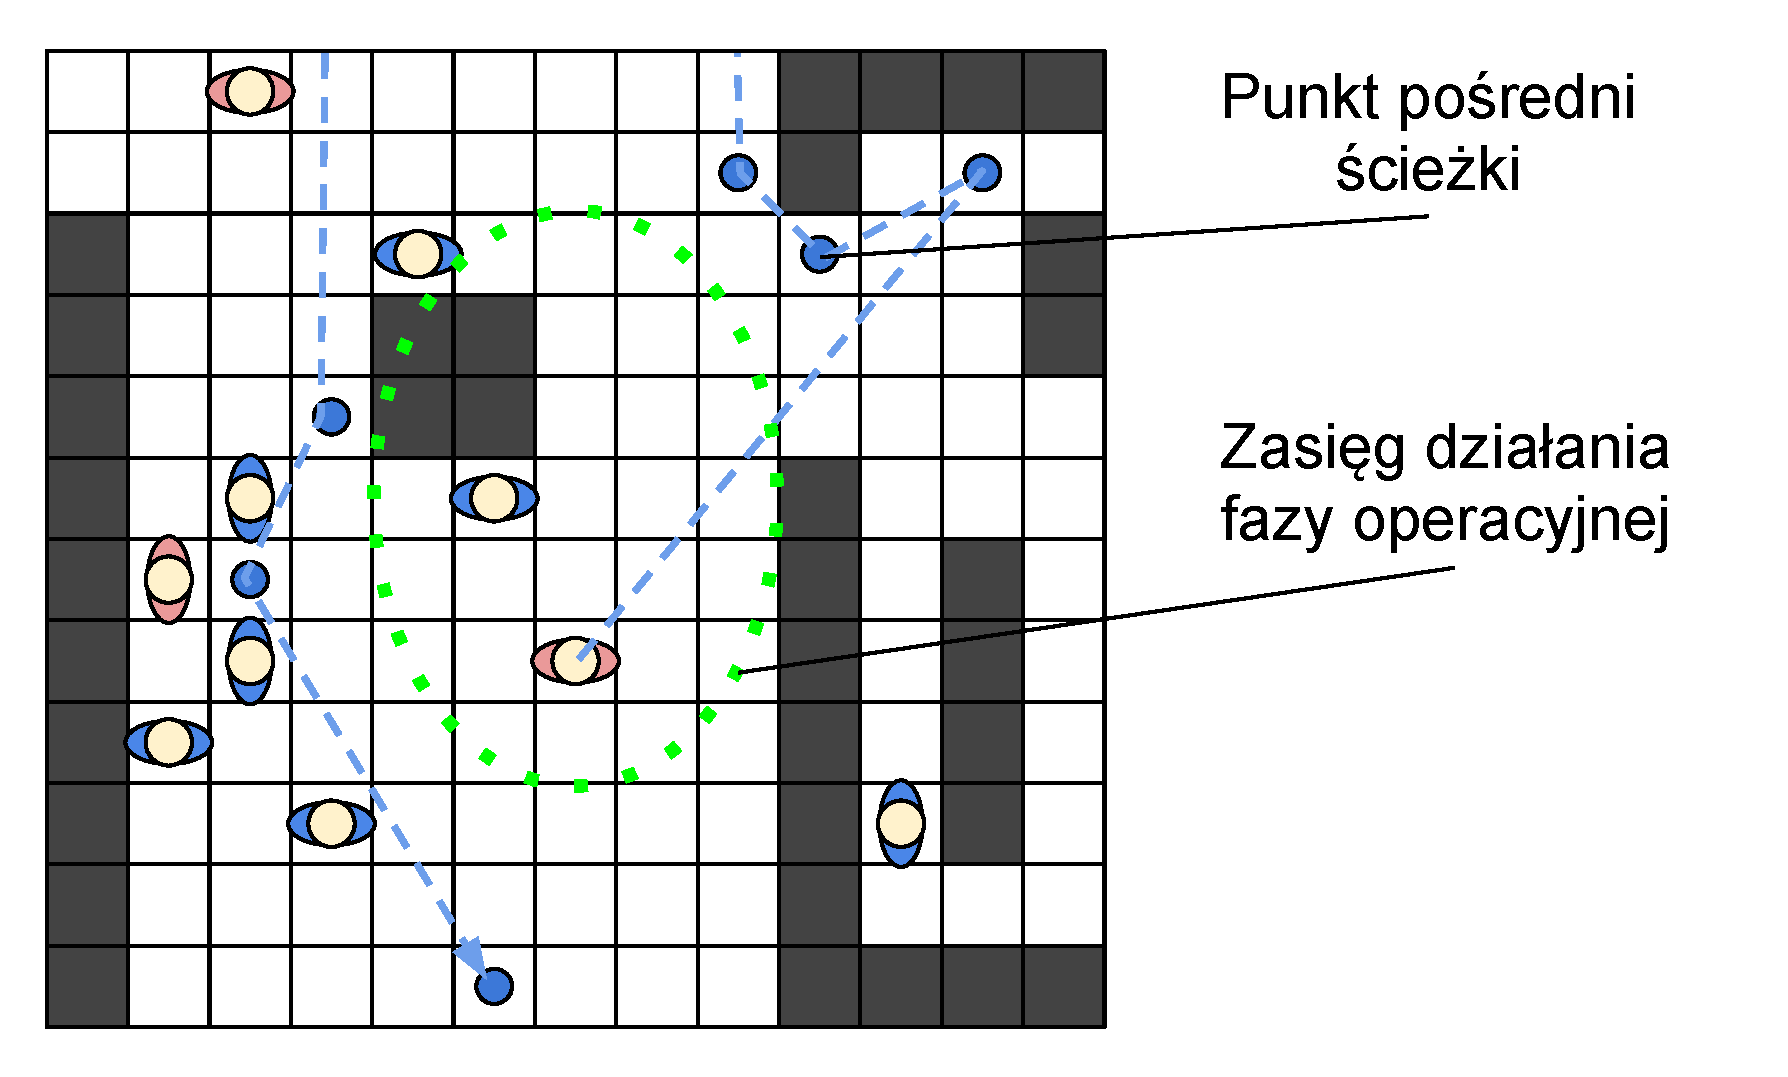
\includegraphics[scale=0.3]{./img/Operative.pdf}
        \end{center}

\noindent
Opis comming soon...

\newpage
    \section{Implementacja}
    \label{sec-3}

     %% TODO
\newpage
    \section{Referencje}
    \label{sec-4}

    %% TODO
\end{document}
